%% LyX 2.3.4.2 created this file.  For more info, see http://www.lyx.org/.
%% Do not edit unless you really know what you are doing.
\documentclass[english,dvipsnames,aspectratio=169]{beamer}
\usepackage{mathptmx}
\usepackage{eulervm}
\usepackage[T1]{fontenc}
\usepackage[latin9]{inputenc}
\usepackage{babel}
\usepackage{amstext}
\usepackage{amssymb}
\usepackage{graphicx}
\usepackage{ifthen}
\usepackage{xcolor}
\usepackage{xspace}
\usepackage{tikz}
\usetikzlibrary{tikzmark}
\usetikzlibrary{calc}
\usepackage{pgfplots}
%\pgfplotsset{compat=1.17}
\usepackage{booktabs}
\usepackage{xpatch}

\xpatchcmd{\itemize}
  {\def\makelabel}
  {\ifnum\@itemdepth=1\relax
     \setlength\itemsep{2ex}% separation for first level
   \else
     \ifnum\@itemdepth=2\relax
       \setlength\itemsep{1ex}% separation for second level
     \else
       \ifnum\@itemdepth=3\relax
         \setlength\itemsep{0.5ex}% separation for third level
   \fi\fi\fi\def\makelabel
  }
 {}
 {}

\ifx\hypersetup\undefined
  \AtBeginDocument{%
    \hypersetup{unicode=true,pdfusetitle,
 bookmarks=true,bookmarksnumbered=false,bookmarksopen=false,
 breaklinks=false,pdfborder={0 0 0},pdfborderstyle={},backref=false,colorlinks=true,
 allcolors=NYUPurple,urlcolor=LightPurple}
  }
\else
  \hypersetup{unicode=true,pdfusetitle,
 bookmarks=true,bookmarksnumbered=false,bookmarksopen=false,
 breaklinks=false,pdfborder={0 0 0},pdfborderstyle={},backref=false,colorlinks=true,
 allcolors=NYUPurple,urlcolor=LightPurple}
\fi

\makeatletter

%%%%%%%%%%%%%%%%%%%%%%%%%%%%%% LyX specific LaTeX commands.
%% Because html converters don't know tabularnewline
\providecommand{\tabularnewline}{\\}

%%%%%%%%%%%%%%%%%%%%%%%%%%%%%% Textclass specific LaTeX commands.
% this default might be overridden by plain title style
\newcommand\makebeamertitle{\frame{\maketitle}}%
% (ERT) argument for the TOC
\AtBeginDocument{%
  \let\origtableofcontents=\tableofcontents
  \def\tableofcontents{\@ifnextchar[{\origtableofcontents}{\gobbletableofcontents}}
  \def\gobbletableofcontents#1{\origtableofcontents}
}

%%%%%%%%%%%%%%%%%%%%%%%%%%%%%% User specified LaTeX commands.
\usetheme{CambridgeUS} 
\beamertemplatenavigationsymbolsempty


% Set Color ==============================
\definecolor{NYUPurple}{RGB}{87,6,140}
\definecolor{LightPurple}{RGB}{165,11,255}


\setbeamercolor{title}{fg=NYUPurple}
\setbeamercolor{frametitle}{fg=NYUPurple}

\setbeamercolor{background canvas}{fg=NYUPurple, bg=white}
\setbeamercolor{background}{fg=black, bg=NYUPurple}

\setbeamercolor{palette primary}{fg=black, bg=gray!30!white}
\setbeamercolor{palette secondary}{fg=black, bg=gray!20!white}
\setbeamercolor{palette tertiary}{fg=gray!20!white, bg=NYUPurple}

\setbeamertemplate{headline}{}
\setbeamerfont{itemize/enumerate body}{}
\setbeamerfont{itemize/enumerate subbody}{size=\normalsize}
\setbeamerfont{itemize/enumerate subsubbody}{size=\normalsize}

\setbeamercolor{parttitle}{fg=NYUPurple}
\setbeamercolor{sectiontitle}{fg=NYUPurple}
\setbeamercolor{sectionname}{fg=NYUPurple}
\setbeamercolor{section page}{fg=NYUPurple}
%\setbeamercolor{description item}{fg=NYUPurple}
%\setbeamercolor{block title}{fg=NYUPurple}

\setbeamertemplate{blocks}[rounded][shadow=false]
\setbeamercolor{block body}{bg=normal text.bg!90!NYUPurple}
\setbeamercolor{block title}{bg=NYUPurple!30, fg=NYUPurple}



\AtBeginSection[]{
  \begin{frame}
  \vfill
  \centering
\setbeamercolor{section title}{fg=NYUPurple}
 \begin{beamercolorbox}[sep=8pt,center,shadow=true,rounded=true]{title}
    \usebeamerfont{title}\usebeamercolor[fg]{title}\insertsectionhead\par%
  \end{beamercolorbox}
  \vfill
  \end{frame}
}

\makeatother

\setlength{\parskip}{\medskipamount} 

\input ../macros

\begin{document}
\input ../rosenberg-macros

\title[DS-GA 1003]{SVM Objective}
\author{He He}
\date{Feb 23, 2021}
\institute{CDS, NYU}

\makebeamertitle
\mode<article>{Just in article version}

\section{Maximum Margin Classifier}

\begin{frame}
    {Linearly Separable Data}
    Consider a linearly separable dataset $\sD$:
    \begin{figure}
        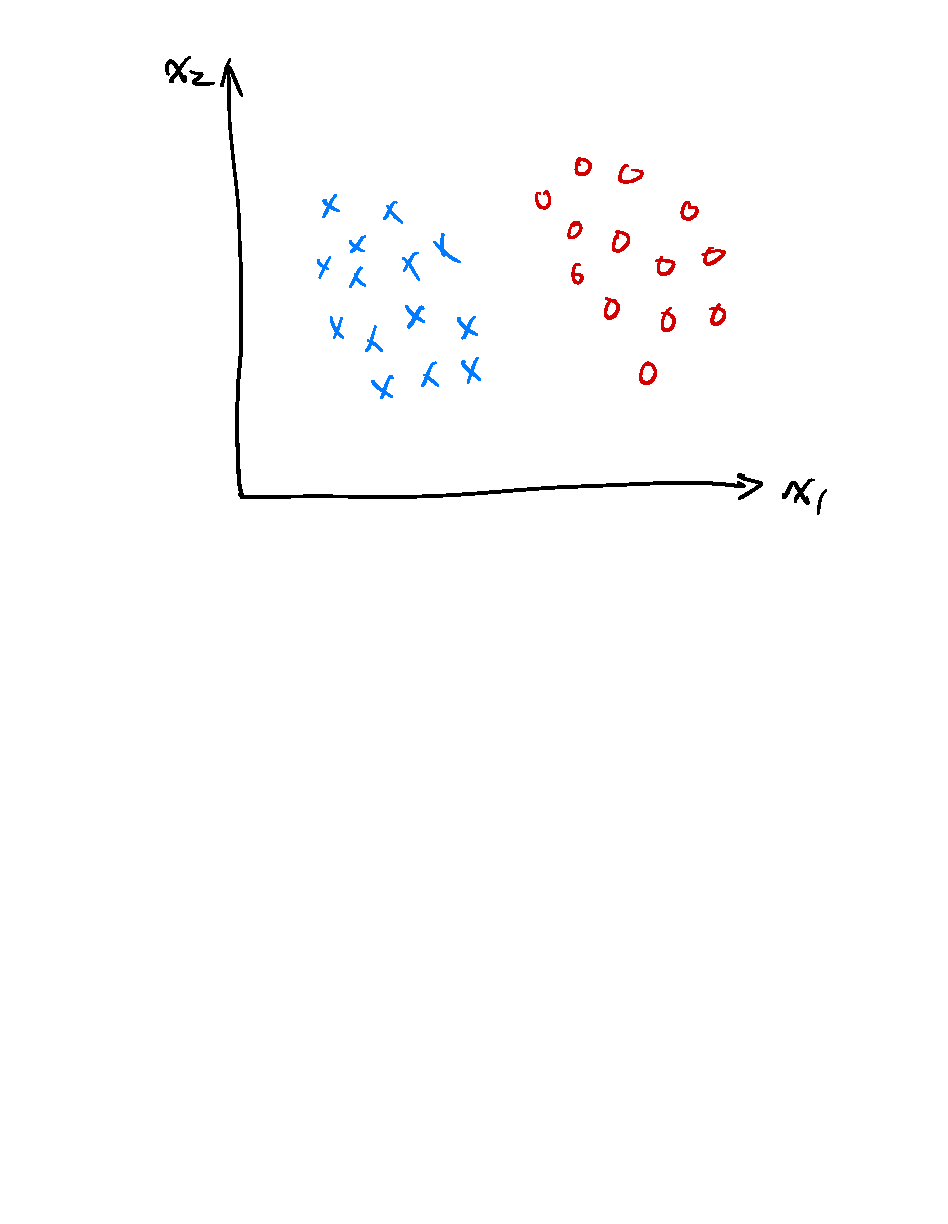
\includegraphics[height=0.5\textheight]{figures/lin-sep-data}
    \end{figure}
    Find a separating hyperplane such that
    \begin{itemize}
        \item $w^Tx_i > 0$ for all $x_i$ where $y_i=+1$
        \item $w^Tx_i < 0$ for all $x_i$ where $y_i=-1$
    \end{itemize}
\end{frame}

\begin{frame}
    {The Perceptron Algorithm}
    \begin{itemize}
        \setlength\itemsep{1ex}
        \item Initialize $w \leftarrow 0$
        \item While not converged (exists misclassified examples)
            \begin{itemize}
                \item For $(x_i, y_i)\in\sD$
                    \begin{itemize}
                        \item If $y_i w^Tx_i < 0$ (wrong prediction)
                        \item Update $w \leftarrow w + y_ix_i$
                    \end{itemize}
            \end{itemize}
    \end{itemize}
    \begin{itemize}
        \item Intuition: move towards misclassified positive examples and away from negative examples
        \item Guarantees to find a zero-error classifier (if one exists) in finite steps
        \item What is the loss function if we consider this as a SGD algorithm?
    \end{itemize}
\end{frame}

\begin{frame}
    {Maximum-Margin Separating Hyperplane}
    For separable data, there are infinitely many zero-error classifiers.

    Which one do we pick?
    \begin{figure}
        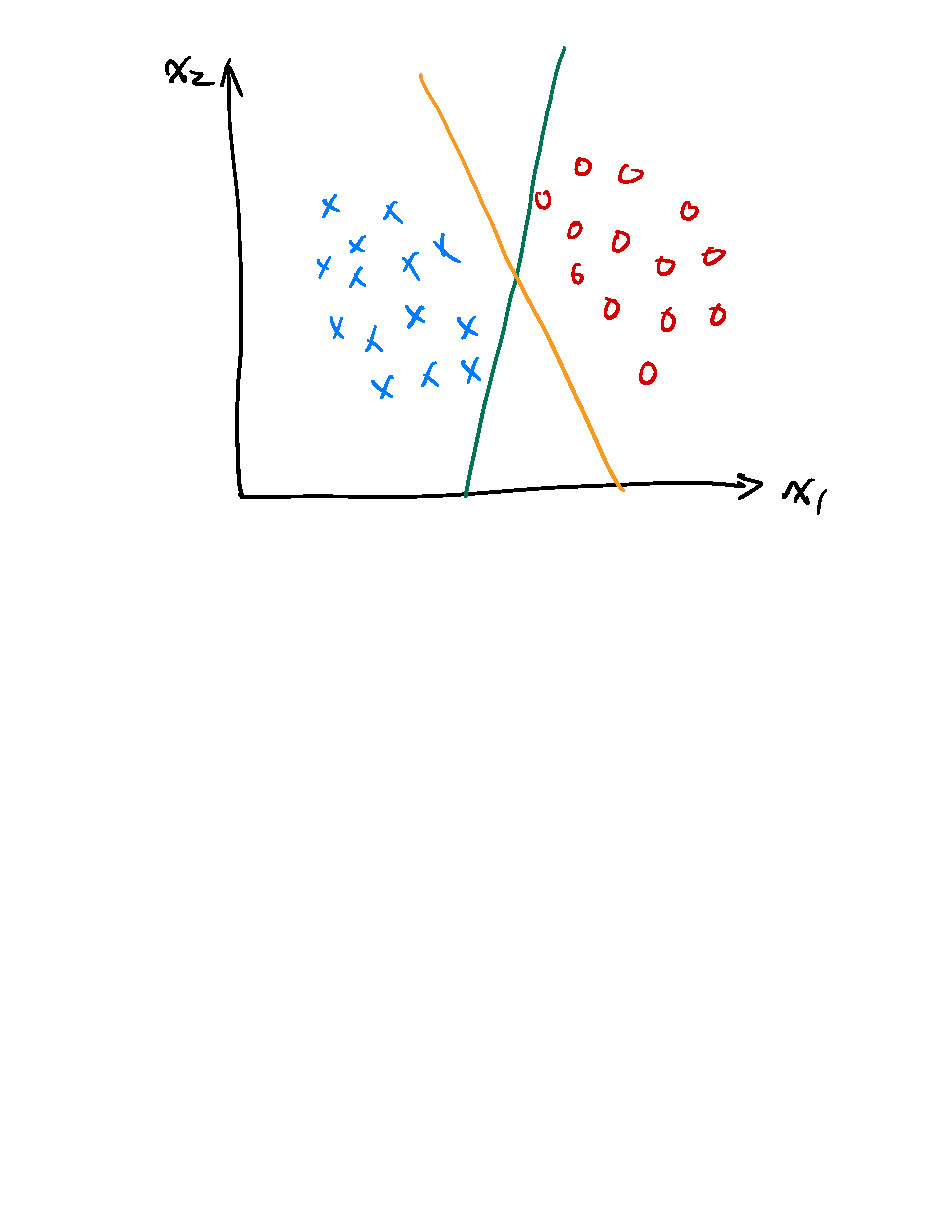
\includegraphics[height=0.5\textheight]{figures/perceptron-hyperplane}
    \end{figure}

    (Perceptron does not return a unique solution.)
\end{frame}

\begin{frame}
    {Maximum-Margin Separating Hyperplane}
    We prefer the classifier that is farthest from both classes of points
    \begin{figure}
        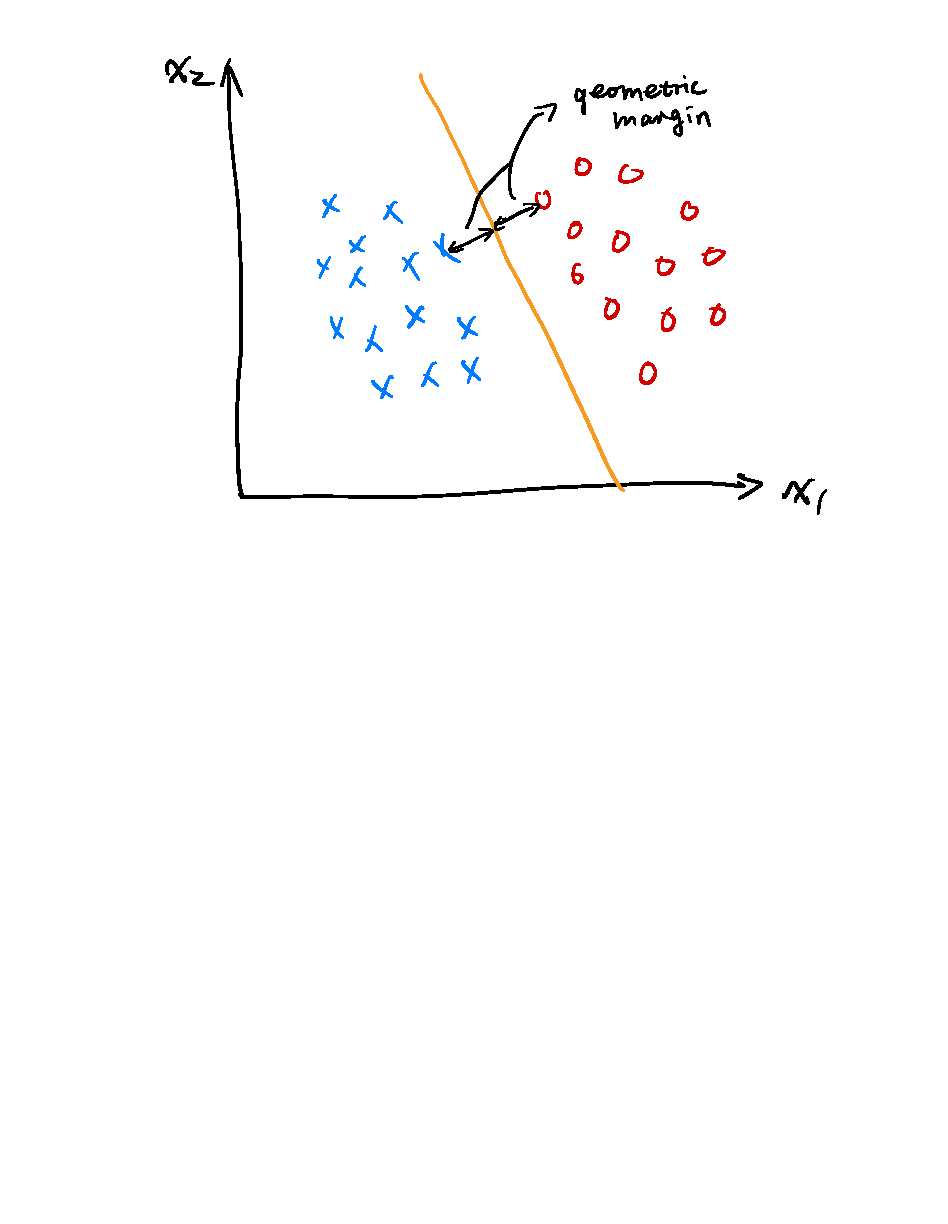
\includegraphics[height=0.5\textheight]{figures/margin}
    \end{figure}
    \begin{itemize}
        \item Geometric margin: smallest distance between the hyperplane and the points 
        \item Maximum margin: \emph{largest} distance to the closest points
    \end{itemize}
\end{frame}

\begin{frame}
    {Geometric Margin}
    We want to maximize the distance between the \hl{separating hyperplane} and the \hl{cloest} points.

    Let's formalize the problem.
    \begin{definition}[separating hyperplane]
    We say $(x_i,y_i)$ for $i=1,\ldots,n$ are \textbf{linearly separable} if there
    is a $w\in\BR^d$ and $b\in\BR$ such that $y_i(w^Tx_i+b)>0$ for all
    $i$. The set $\{v\in\BR^d\mid w^Tv+b=0\}$ is called a \textbf{separating hyperplane}.    
  \end{definition}

    \begin{definition}[geometric margin]
        Let $H$ be a hyperplane that separates the data $(x_i,y_i)$ for $i = 1,\ldots,n$. The \textbf{geometric margin} of this hyperplane is
        $$
        \min_i d(x_i, H),
        $$
    the distance from the hyperplane to the closest data point.
    \end{definition}
\end{frame}

\begin{frame}
    {Distance between a Point and a Hyperplane}
    \vspace{10em}
    \begin{itemize}
        \item Projection of $v\in\BR^d$ onto $w\in\BR^d$:
            $\frac{v\cdot w}{\|w\|_2}$
        \item Distance between $x_i$ and $H$:
            $$
            d(x_i, H) = \left |\frac{w^Tx_i + b}{\|w\|_2}\right |
            = \frac{y_i(w^Tx_i + b)}{\|w\|_2}
            $$
    \end{itemize}
\end{frame}

\begin{frame}
    {Maximize the Margin}
    We want to maximize the geometric margin:
    $$
    \text{maximize} \; \min_{i} d(x_i, H) .
    $$
    Given separating hyperplane $H=\pc{v\mid w^Tv + b = 0}$, we have
    $$
    \text{maximize} \; \min_{i} \frac{y_i(w^Tx_i + b)}{\|w\|_2} .
    $$
    Let's remove the inner minimization problem by
      $$\begin{array}{ll}
      \text{maximize} & M\\
          \text{subject to} & \frac{y_i(w^Tx_i+b)}{\|w\|_2} \geq M \quad\text{for all
        $i$}
    \end{array}$$
    Note that the solution is not unique (why?).
\end{frame}

\begin{frame}
    {Maximize the Margin}
    Let's fix the norm $\|w\|_2$ to $1/M$ to obtain:
      $$\begin{array}{ll}
          \text{maximize} & \frac{1}{\|w\|_2}\\
      \text{subject to} & y_i(w^Tx_i+b) \geq 1 \quad\text{for all
        $i$}
    \end{array}$$
    It's equivalent to solving the minimization problem
      $$\begin{array}{ll}
          \text{minimize} & {\frac{1}{2}\|w\|_2^2}\\
      \text{subject to} & y_i(w^Tx_i+b) \geq 1 \quad\text{for all
        $i$}
    \end{array}$$

    Note that $y_i(w^Tx_i+b)$ is the (functional) margin.

    In words, it finds the minimum norm solution which has a margin of at least 1 on all examples.
\end{frame}

\begin{frame}
    {Soft Margin SVM}
    What if the data is \textit{not} linearly separable?

    For any $w$, there will be points with a negative margin.

    Introduce \textbf{slack variables} to penalize small margin:
      $$\begin{array}{ll}
          \text{minimize} & {\frac{1}{2}\|w\|_2^2}
           + \frac{C}{n}\sum_{i=1}^n \xi_i \\
      \text{subject to} & y_i(w^Tx_i+b) \geq 1 - \xi_i \quad\text{for all
        $i$}\\
          & \xi_i \geq 0 \quad\text{for all $i$}
    \end{array}$$
    \begin{itemize}
        \setlength\itemsep{1ex}
        \item If $\xi_i = 0 \;\forall i$, it's reduced to hard SVM.
        \item What does $\xi_i > 0$ mean?
        \item What does $C$ control?
    \end{itemize}
\end{frame}

\begin{frame}
    {Slack Variables}
    $d(x_i, H) = \frac{y_i(w^Tx_i+b)}{\|w\|_2} \ge \frac{1-\xi_i}{\|w\|_2}$,
    thus $\xi_i$ measures the violation by multiples of the geometric margin:
    \begin{itemize}
        \setlength\itemsep{1ex}
        \item $\xi_i=1$: $x_i$ lies on the hyperplane
        \item $\xi_i=3$: $x_i$ is past 2 margin width beyond the decision hyperplane 
    \end{itemize}
    \begin{figure}
        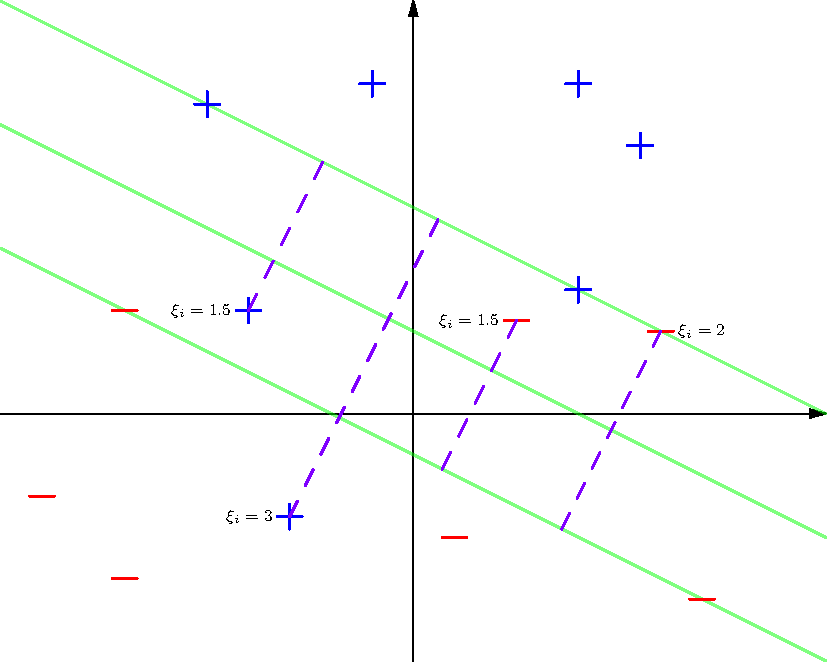
\includegraphics[height=0.6\textheight]{figures/SoftMargin}
    \end{figure}
\end{frame}

\section{Minimize the Hinge Loss}
\begin{frame}
    {Perceptron Loss}
    $$
    \ell(x,y,w) = \max(0, -yw^Tx)
    $$
    \begin{figure}
        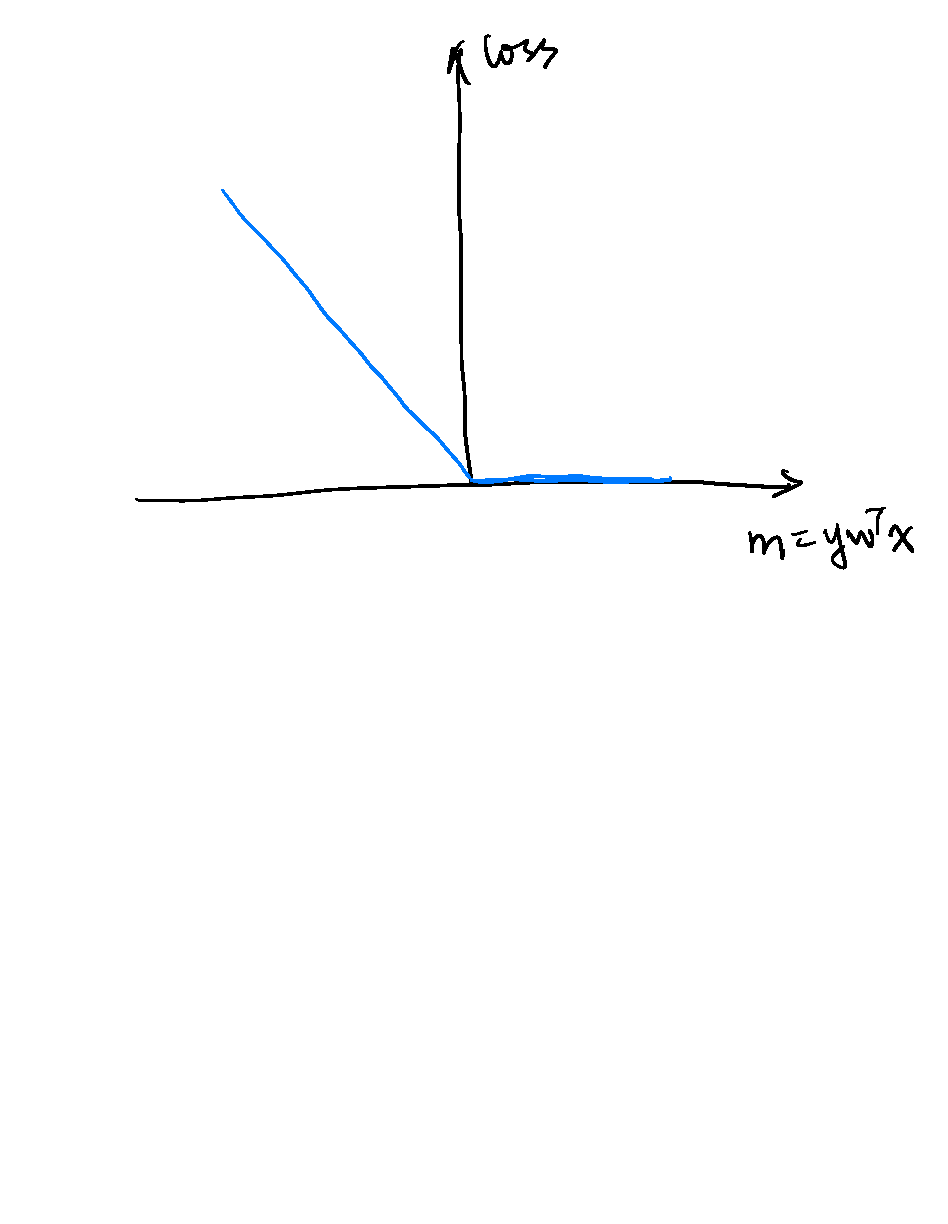
\includegraphics[height=0.5\textheight]{figures/perceptron-loss}
    \end{figure}
    If we do ERM with this loss function, what happens?
\end{frame}

\begin{frame}{Hinge Loss}
\begin{itemize}
\item SVM/Hinge loss: $\loss_{\text{Hinge}}=\max\left\{ 1-m,0\right\} =\left(1-m\right)_{+}$
\item Margin $m=yf(x)$; ``Positive part'' $(x)_{+}=x\ind{x\ge0}$.
\end{itemize}
\begin{center}
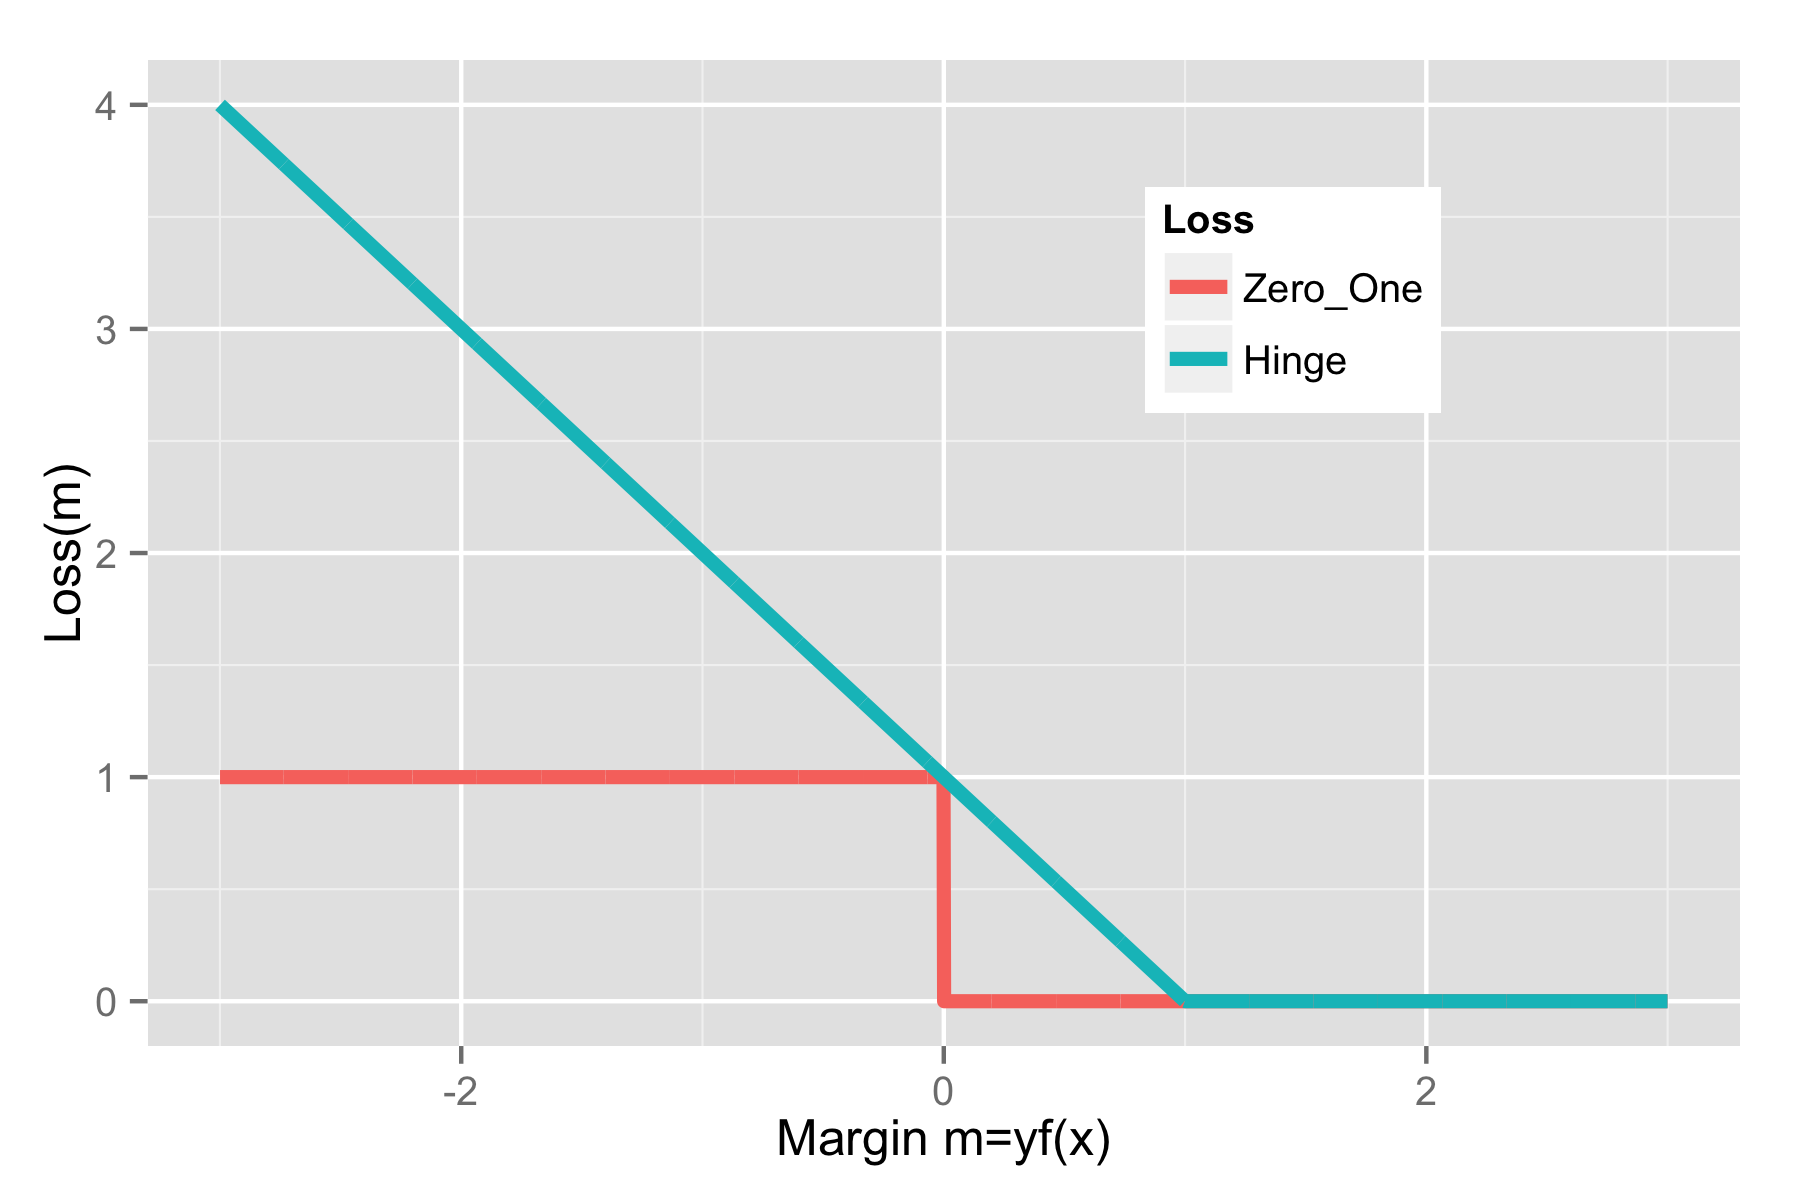
\includegraphics[height=0.5\textheight]{figures/loss.Zero_One.Hinge}
\par\end{center}

Hinge is a \textbf{convex}, \textbf{upper bound} on $0-1$ loss. Not
differentiable at $m=1$. \\
We have a \textbf{``margin error''} when $m<1$.
\end{frame}

\begin{frame}{Support Vector Machine}
    Using ERM:
\begin{itemize}
\item Hypothesis space $\cf=\left\{ f(x)=w^{T}x+b\mid w\in\reals^{d},b\in\reals\right\} $.
\item $\ell_{2}$ regularization (Tikhonov style)
\item Hinge loss $\ell(m)=\max\left\{ 1-m,0\right\} =\left(1-m\right)_{+}$
\item The SVM prediction function is the solution to
\[
\min_{w\in\reals^{d},b\in\reals}\frac{1}{2}||w||^{2}+\frac{c}{n}\sum_{i=1}^{n}\max\left(0,1-y_{i}\left[w^{T}x_{i}+b\right]\right).
\]
\item \al{Not differentiable} because of the $\max$
\end{itemize}
\end{frame}

\begin{frame}{SVM as a Constrained Optimization Problem}
\begin{itemize}
\item The SVM optimization problem is equivalent to
\begin{eqnarray*}
    \textrm{minimize} &  & \frac{1}{2}||w||^{2}+\frac{c}{n}\sum_{i=1}^{n}\xi_{i}\\
\textrm{subject to} &  & \xi_{i}\ge\max\left(0,1-y_{i}\left[w^{T}x_{i}+b\right]\right).
\end{eqnarray*}


\item Which is equivalent to
\begin{eqnarray*}
    \textrm{minimize} &  & \frac{1}{2}||w||^{2}+\frac{c}{n}\sum_{i=1}^{n}\xi_{i}\\
\textrm{subject to} &  & \xi_{i}\ge\left(1-y_{i}\left[w^{T}x_{i}+b\right]\right)\;\mbox{for }i=1,\ldots,n\\
 &  & \xi_{i}\ge0\;\mbox{for }i=1,\ldots,n
\end{eqnarray*}
\end{itemize}
\end{frame}

\begin{frame}
    {Summary}
    Two ways to derive the SVM optimization problem:
    \begin{itemize}
    \item Maximize the (geometric) margin
    \item Minimize the hinge loss with $\ell_2$ regularization
    \end{itemize}
    Both leads to the minimum norm solution satisfying certain margin constraints.

    \begin{itemize}
        \item \textbf{Hard-margin SVM}: all points must be correctly classified with the margin constraints
        \item \textbf{Soft-margin SVM}: allow for margin constraint violation with some penalty
    \end{itemize}
\end{frame}

\end{document}
